% !TeX spellcheck = cs_CZ
%{\tikzset{external/prefix={tikz/FYZI/}}
% \tikzset{external/figure name/.add={ch51_}{}}
%---------------------------------------------------------------------------------------------------
% file fey1ch51.tex
%---------------------------------------------------------------------------------------------------
%=========================== Kapitola: Vlny ========================================================
\setchaptertoc
\chapter{Vlny}\label{fyz:IchapLI}

\section{Kuželové vlny}\label{fyz:IchapLIsecI}
  I když jsme už skončili kvantitativní analýzu vln, věnujeme tuto doplňkovou kapitolu 
  kvalitativnímu posouzení některých jevů souvisejících s vlnami, které jsou příliš složité na to, 
  abychom je mohli v těchto přednáškách podrobně prozkoumat.
  
  Protože jsme už několik kapitol věnovali vlnám, bylo by přiměřenější nazvat tuto kapitolu 
  kapitolou o „některých složitějších jevech souvisejících s vlnami“.
  
  \begin{figure}[ht!] %\ref{fyz:fig0386}
    \centering
    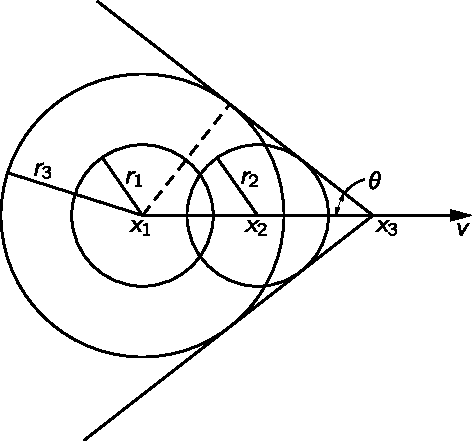
\includegraphics[width=0.6\linewidth]{fyz_fig0386.pdf}
    \caption{Čelo rázové vlny vytváří kužel s vrcholem ve zdroji a s polovičním úhlem rozevření
             \(\alpha =\arcsin(v/c_v)\)
             (\cite[s.~686]{Feynman01})}
    \label{fyz:fig0386}
  \end{figure}

  Prvním předmětem našich úvah bude jev, který vzniká tehdy, když se zdroj vln pohybuje větší 
  rychlostí, než je rychlost vlny nebo fázová rychlost. Uvažujme nejprve vlny jako zvuk nebo 
  světlo, které mají určitou konstantní rychlost. Je-li rychlost pohybu zdroje zvuku větší než 
  rychlost zvuku, nastává následující jev. Předpokládejme, že v daném okamžiku je zvuková vlna 
  vybuzena zdrojem v bodě \(x_1\) (viz obr. \ref{fyz:fig0386}). Potom v dalším okamžiku, kdy se 
  zdroj dostane do bodu \(x_2\), se vlna rozšíří z bodu \(x_1\) na kulovou plochu poloměru \(r_1\), 
  který je menší než vzdálenost, jíž prošel zdroj. Z bodu \(x_2\), se ovšem začne šířit další vlna. 
  Dostal-li se zvukový zdroj ještě dále, až do bodu \(x_3\) a z tohoto bodu vychází další vlna, 
  vlna z \(x_2\) se rozšířila na kulovou plochu poloměru \(r_2\) a vlna z \(x_1\) poloměru \(r_3\). 
  Děje se to samozřejmě spojitě, a ne skoky, a proto máme celou řadu takových kulových vlnoploch 
  dotýkajících se pláště kužele s vrcholem v místě zdroje. Místo toho, aby zdroj vytvářel kulové 
  vlny, jako v případě, kdyby se nepohyboval, vytváří pohybující se zdroj vlny, jejichž čelo je v 
  trojrozměrném prostoru kužel a v dvojrozměrném prostoru dvojice přímek. Vrcholový úhel tohoto 
  kužele lze snadno určit. V určitém časovém intervalu projde zdroj vzdálenost např. \(x_3 - x_1\), 
  která je úměrná rychlosti vlny \(c_v\). Je jasné, že sinus polovičního úhlu rozevření kužele je 
  roven poměru rychlosti vlny k rychlosti zdroje a to je možné jen tehdy, když \(c_v\) menší než 
  \(v\), tedy když se předmět pohybuje rychleji než vlna. Proto
  \begin{equation}\label{fyz:eq527}
    \sin\theta = \dfrac{c_v}{v}
  \end{equation}
  
  \begin{figure}[ht!] %\ref{fyz:fig0387}
    \centering
    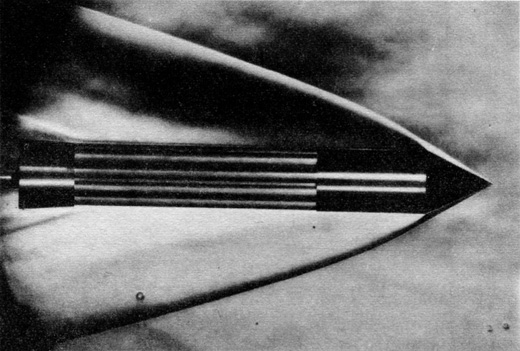
\includegraphics[width=0.6\linewidth]{fyz_fig0387.jpg}
    \caption{Rázová vlna vyvolaná v plynu projektilem pohybujícím se rychleji než zvuk
             (\cite[s.~687]{Feynman01})}
    \label{fyz:fig0387}
  \end{figure}
  
  I když jsme zdůraznili, že máme \emph{zdroj} zvuku, ukazuje se - a to je velmi zajímavé - že 
  předmět už tím, že se pohybuje rychlostí větší než je rychlost zvuku, \emph{vytváří} zvuk. To 
  znamená, že on sám nemusí kmitat. Jakýkoliv objekt pohybující se prostředím větší rychlostí než 
  je rychlost, kterou se v tom prostředí šíří vlny, bude vytvářet automaticky vlny právě v důsledku 
  svého rychlého pohybu. Tak je to v případě zvuku, ale stejný jev nastává i v případě světla. Na 
  první pohled by se zdálo, že se nic nemůže pohybovat rychlostí větší než je rychlost světla. 
  Jenže světlo má ve skle menší fázovou rychlost, než je rychlost světla ve vakuu a sklem můžeme 
  propustit nabitou částici s velmi vysokou energií, takže rychlost částice bude blízká rychlosti 
  světla ve vakuu, zatímco rychlost světla ve skle může být rovna jen 2/3 rychlosti světla ve 
  vakuu. Částice pohybující se rychleji než světlo v daném prostředí vytvoří kuželovou světelnou 
  vlnu s vrcholem ve zdroji, která se podobá vlně vznikající na vodě za lodí (jde vlastně o stejný 
  jev). Změřením úhlu u vrcholu kužele můžeme určit rychlost částice. Takový postup se používá v 
  praxi k měření rychlosti částic jako jedna z metod určování jejich energie ve vysokoenergetické 
  oblasti. Jediné, co je třeba měřit, je směr šíření světla. 
  
  Tento jev se nazývá podle Čerenkova, který jej poprvé pozoroval. Intenzitu tohoto záření 
  teoreticky analyzovali Frank a Tamm. Za tento výzkum dostali tito tři vědci společně Nobelovu 
  cenu za fyziku v roce 1958.
  
  Na obrázku \ref{fyz:fig0387} můžete vidět, jaká je situace v případě zvuku. Je to fotografie 
  předmětu pohybujícího se v plynu rychlostí, která je větší než rychlost zvuku. Změny tlaku 
  způsobují změny indexu lomu, takže vhodnou optickou soustavou můžeme okraj vln zviditelnit. Tak 
  vidíme, že předmět pohybující se rychlostí, která je větší než je rychlost zvuku, opravdu vytváří 
  kuželovou vlnu. Podrobnější zkoumání nás přesvědčí o tom, že její povrch je vlastně zakřivený. V 
  asymptotické oblasti není zakřivení, ale u vrcholu zakřivení existuje a my bychom si nyní měli 
  promluvit o příčině tohoto zakřivení. To nás přivádí k druhému tématu této kapitoly.
  
\section{Rázové vlny}\label{fyz:IchapLIsecII}
  Rychlost vlny často závisí na její amplitudě a v případě zvuku má tato závislost následující 
  charakter. Předmět, který se pohybuje ve vzduchu, musí odstraňovat vzduch ze své dráhy, a tak 
  vytváří poruchu ve formě určitého tlakového skoku. Tlak za čelem vlny je vyšší než tlak v 
  neporušené oblasti, do níž se vlna pohybující se normální rychlostí ještě nedostala. Avšak 
  vzduch, který zůstal za vlnou, byl adiabaticky stlačen, a proto jeho teplota bude vyšší. Rychlost 
  zvuku však s teplotou roste, a proto je rychlost v oblasti za skokem větší než ve vzduchu před 
  skokem. To znamená, že jakákoliv další porucha za tímto skokem, vyvolaná třeba stálým tlakem 
  tělesa nebo jinak, se bude šířit rychleji než čelo vlny a s růstem tlaku tato rychlost poroste. 
  Obr. \ref{fyz:fig0388} charakterizuje takovou situaci a hrboly na křivce tlaku slouží větší 
  názornosti. Je vidět, že původní zadní oblasti vyššího tlaku postupem času dobíhají čelo vlny, 
  dokud tlaková vlna nevytvoří strmé čelo.Je-li síla vlny velmi velká, stane se to ihned; je-li 
  malá, může to trvat dlouho. Ve skutečnosti se však může stát, že zvuk se rozšíří a zanikne dříve, 
  než k takovému jevu dojde.
  \begin{figure}[ht!] %\ref{fyz:fig0388}
    \centering
    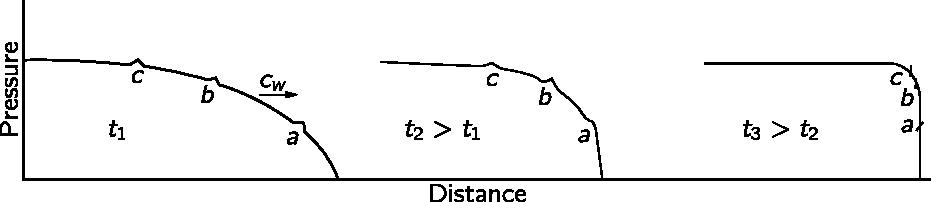
\includegraphics[width=0.9\linewidth]{fyz_fig0388.pdf}
    \caption{\uv{Momentky} čela vlny v následujících časových okamžicích
             (\cite[s.~688]{Feynman01})}
    \label{fyz:fig0388}
  \end{figure}
  
  Zvuky naší řeči jsou nesmírně slabé vzhledem k atmosferickému tlaku - je to asi jedna milióntina. 
  Ale pro tlakové změny řádově jedné atmosféry vzroste rychlost vlny asi o dvacet procent a strmost 
  čela vlny naroste úměrně rychleji. V přírodě se však nic neděje \emph{nekonečně} rychle, a to, co 
  nazýváme strmým čelem, má ve skutečnosti přece jen jakousi tloušťku, není to nekonečně strmé. 
  Vzdálenost, na níž se čelo mění, je řádově rovna střední volné dráze, ale na takové vzdálenosti 
  vlnová rovnice neplatí, neboť neuvažujeme strukturu plynu.
  
  Podíváme-li se opět na obrázek \ref{fyz:fig0387}, zjistíme, že zakřivení můžeme vysvětlit tím, že 
  v blízkosti vrcholu jsou vyšší tlaky než ve větší vzdálenosti od něho, a proto je tam úhel 
  \(\theta\) větší. Zakřivení vzniklo v důsledku toho, že rychlost závisí na síle vlny. Proto se 
  vlna pocházející od výbuchu atomové bomby šíří po určitou dobu mnohem větší rychlostí, než je 
  rychlost zvuku, dokud při šíření natolik nezeslábne, že tlakový náraz je malý ve srovnání s 
  atmosférickým tlakem. Rychlost tlakového nárazu se pak přiblíží rychlosti zvuku v plynu, v němž 
  se šíří. (Ukazuje se, že rychlost rázové vlny je vždy vyšší než rychlost zvuku v plynu před ní, 
  ale nižší než rychlost zvuku v plynu za ní. Impulzy přicházející zezadu doběhnou čelo, ale čelo 
  se noří do prostředí před sebou rychleji, než je normální rychlost šíření signálů v něm. Proto 
  jen podle zvuku nemůžeme říci, že přichází rázová vlna, dokud není příliš pozdě. Světlo výbuchu 
  bomby přichází nejdříve, ale že přichází rázová vlna, nemůže nikdo říci, dokud vlna opravdu 
  nedorazí, protože ji nepředchází žádný zvukový signál.)
  
  \begin{figure}[ht!] %\ref{fyz:fig0389}
    \centering
    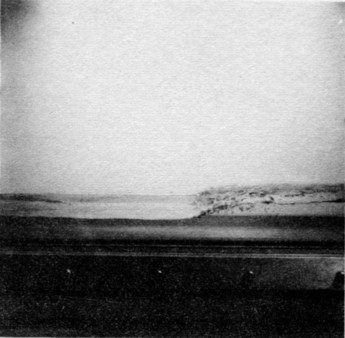
\includegraphics[width=0.6\linewidth]{fyz_fig0389.jpg}
    \caption{
             (\cite[s.~689]{Feynman01})}
    \label{fyz:fig0389}
  \end{figure}
  
  Takové nahromadění vln je velmi zajímavý jev a jeho hlavní příčinou je to, že po příchodu jedné 
  vlny musí rychlost po ní následující vlny vzrůstat. Uvedeme ještě jiný příklad téhož jevu. 
  Představme si, že dlouhým kanálem konečné šířky a hloubky teče voda. Pohybuje-li se podél 
  takového kanálu dostatečně rychle píst nebo příčná stěna, dojde k takovému nakupení vody jako v 
  případě sněhu před sněžným pluhem. Nechť tedy nastává taková situace, jakou zobrazuje obrázek 
  \ref{fyz:fig0389}, kdy se někde v kanálu objevuje náhlý skok vodní hladiny. Lze ukázat, že v 
  kanálu se dlouhé vlny pohybují v hluboké vodě rychleji než v mělké. Proto každý nový náraz nebo 
  nepravidelnost v přísunu energie od pístu postoupí dopředu a nahromadí se na čele. Teoretický 
  nakonec opět dostaneme vodu se strmým čelem. Obrázek \ref{fyz:fig0389} však ukazuje na některé 
  komplikace. Znázorněná vlna prochází na obrázku kanálem tak, že píst je kdesi daleko na levé 
  straně. Zpočátku mohla situace připomínat dobře se chovající vlnu, ale na cestě podél kanálu se 
  vlna stávala strmější a strmější, až došlo ke stavu znázorněnému na obrázku. Na hladině dochází k 
  silnému víření vody a kapky vody padají dolů. ale podstatně je, že okraj vlny je velmi ostrý a 
  před vlnou není voda porušena.  
  
  Ve skutečnosti je vlna na vodě mnohem složitější než zvuk. Pro ilustraci se však pokusíme 
  analyzovat rychlost přílivové vlny v kanálu. Neděláme to proto, že by to pro nás mělo 
  principiální význam - nepředstavuje to totiž velké zobecnění - děláme to jenom proto, abychom 
  ukázali, že zákony mechaniky, které už známe, nám umožní tento jev vysvětlit. 
  
  \begin{figure}[ht!] %\ref{fyz:fig0390}
    \centering
    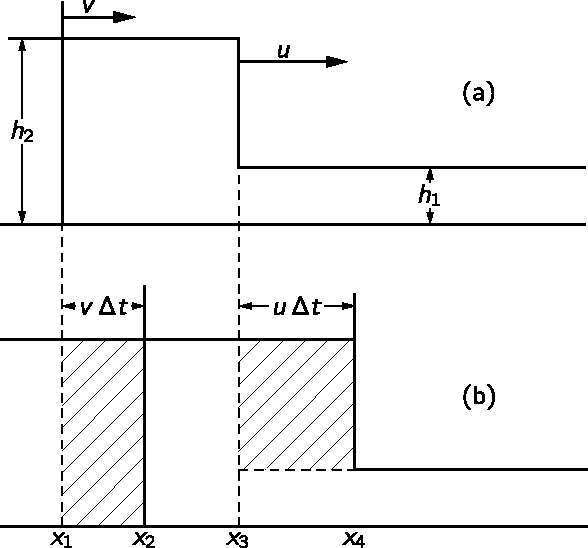
\includegraphics[width=0.6\linewidth]{fyz_fig0390.pdf}
    \caption{Dva průřezy vysokého přílivu v kanálu, kde b) je obraz situace o \(\Delta t\)
                 pozdější než a)
             (\cite[s.~689]{Feynman01})}
    \label{fyz:fig0390}
  \end{figure}
  
  Představme si, že voda vypadá tak, jako znázorňuje obrázek \ref{fyz:fig0390}a na horní hladině ve 
  výšce \(h_2\) se pohybuje rychlostí \(v\) a čelo se posouvá rychlostí \(u\) na neporušenou vodu, 
  jejíž hladina je ve výšce \(h_1\). Chceme určit rychlost, kterou postupuje čelo. Za dobu \(\Delta 
  t\) se vertikální rovina, která byla původně v \(x_1\), posune o vzdálenost \(v\Delta t\) do 
  \(x_2\), zatímco čelo vlny projde vzdálenost \(u\Delta t\).
  
  Nyní použijeme zákony zachování hmotnosti a hybnosti. Začneme prvním z nich. Je vidět že na 
  jednotku šířky kanálu je množství vody \(h_2v\Delta t\), které prošlo \(x_1\) (vyšrafovaná 
  oblast), kompenzováno druhou vyšrafovanou oblastí, jež představuje množství \((h_2-h_1)u\Delta 
  t\). Dělíme-li veličinou \(\Delta t\), dostaneme \(vh_2=u(h_2-h_1)\) To nám ještě nestačí, 
  protože i když známe \(h_2\) a \(h_1\), neznáme ani \(u\) ani \(v\) a obě tyto veličiny chceme 
  najít. 
  
  Dalším krokem je použití zákona zachování hybnosti. Nezabývali jsme se ještě otázkou vodního 
  tlaku a nemluvili jsme o hydrodynamice, ale je jasné, že tlak vody musí v dané hloubce právě 
  stačit k udržení vodního sloupce nad touto hloubkou. Proto je tlak vody roven součinu hustoty 
  vody \(\varrho\), gravitačního zrychlení \(g\) a hloubky pod povrchem. Protože tlak roste 
  lineárně s hloubkou, střední tlak v rovině \(x_1\) je právě \(1/2\varrho gh_2\). To je také 
  střední síla na jednotku šířky a jednotku výšky tlačící rovinu směrem k \(x_2\). Abychom dostali 
  celkovou sílu působící na vodu zleva, musíme získaný výraz znovu násobit \(h_2\). Na vodu však 
  působí i tlak zprava a vyvolává sílu, která na uvažovanou oblast působí v opačném směru. Podobnou 
  úvahou jako v předcházejícím případě můžeme vypočítat její velikost: \(1/2\varrho gh_1^2\). Nyní 
  musíme tyto síly porovnat s rychlostí změny hybnosti pohybu. Musíme zjistit, o kolik je větší 
  hybnost odpovídající situaci (b) na obr. \ref{fyz:fig0390} proti hybnosti odpovídající situaci 
  (a). Vidíme, že dodatečná hmotnost, která získala rychlost \(v\) je rovna právě \(\varrho 
  h_2u\Delta t - \varrho h_2v\Delta t\) (na jednotku šířky) a násobíme-li ji \(v\), dostaneme 
  dodatečnou hybnost, která musí být rovna impulzu \(F\Delta t\)
  \begin{equation*}
    (\varrho h_2u\Delta t - \varrho h_2v\Delta t) v
      = \left(\dfrac{1}{2}\varrho g h_2^2 - \dfrac{1}{2}\varrho g h_1^2\right)\Delta t.
  \end{equation*}
  Dosazením už známého vztahu \(vh_2 = u(h_2 - h_1)\) vyloučíme z této rovnice \(v\), a když ji 
  ještě zjednodušíme, dostaneme nakonec: \(u^2 = gh_2(h_1 + h_2)-gh (h+h)/2 h_1\).
  
  Je-li rozdíl výšek velmi malý, takže \(h_1\), a \(h_2\) jsou téměř stejné, rychlost bude rovna 
  \(\sqrt{gh}\). Později uvidíme, že to platí jen tehdy, je-li vlnová délka vlny větší než hloubka 
  kanálu.
  
  Obdobně můžeme postupovat i v případě rázových vln, ale je třeba uvažovat zachování vnitřní 
  energie, a ne entropie, protože rázová vlna představuje nevratný děj. Opravdu, kdybychom 
  ověřovali platnost zákona zachování energie v případě přílivové vlny, zjistili bychom, že tento 
  zákon není splněn. Jsou-li výškové rozdíly malé, je jeho narušení zanedbatelné, ale v případě 
  velkých výškových rozdílů jsou značné energetické ztráty. Projevuje se to pádem vody a zpěněním 
  znázorněným na obr. \ref{fyz:fig0389}.
  
  
  I v případě rázových vln se z hlediska adiabatických procesů také vyskytují ztráty energie. 
  Energie zvukové vlny za čelem po průchodu vlny zahřívá plyn, což odpovídá zpěnění vody při 
  přílivu. Ukazuje se, že v případě zvuku je třeba řešit tři rovnice, a jak jsme viděli, teplota za 
  rázovou vlnou je jiná než teplota před ní.
  
  Kdybychom se pokusili vytvořit převrácenou přílivovou vlnu, kdy h<h, zjistili bychom, že 
  energetické ztráty musí být záporné. Protože energie není odnikud k dispozici, takový typ přílivu 
  se nemůže sám udržet je nestabilní. Kdybychom začali tvořit vlnu takového typu, zploštila by se, 
  protože závislost rychlosti na výšce, která vytvářela v předcházejícím případě strmé čelo, bude 
  nyní právě opačná.

\section{Vlny v pevných látkách}\label{fyz:IchapLIsecIII}
  Dalším složitějším typem vln, o nichž budeme mluvit, jsou vlny v pevných látkách. Už jsme mluvili 
  o zvukových vlnách v plynu a kapalině a tyto vlny mají analogii ve vlnách šířících se v pevných 
  látkách. Při nárazu na pevné těleso dojde k jeho stlačení. Pevná látka se však tomuto stlačení 
  brání a tak vznikne vlna podobná zvuku. V pevné látce však může existovat i takový druh vln, 
  který neexistuje v tekutinách. Zdeformujeme-li pevné těleso tečnými silami, smykem, bude se 
  snažit vrátit do původního stavu. Právě tím se liší podle definice pevná látka od kapaliny. 
  Narušíme-li kapalinu (vnitřně), chvíli ji necháme, aby se uklidnila a pak na ni přestaneme 
  působit, zůstane v nově nabytém stavu. Vezmeme-li pevné těleso a roztřeseme ho jako kus želé, 
  začne se v něm šířit příčná vlna postupující tělesem podobně jako vlna stlačení. Rychlost příčné 
  vlny je však vždy menší než rychlost podélné vlny - vlny stlačení. Příčné vlny se víc podobají, 
  alespoň pokud jde o jejich polarizaci, světelným vlnám. Zvuk nemá žádnou polarizaci, je to prostě 
  tlaková vlna. Světlo má charakteristickou orientaci kolmou ke směru šíření. 
  
  V pevné látce existují oba druhy vln. Je tam především vlna stlačení, analogická zvuku, která se 
  šíří jednou rychlostí. Není-li pevná látka krystal, šíří se v ní charakteristickou rychlostí 
  libovolným směrem polarizovaná příčná vlna. (Všechny pevné látky jsou krystalické, ale máme-li 
  kousek skládající se z mikrokrystalů všech orientací, krystalová anizotropie se vykompenzuje.) 
  
  \begin{figure}[ht!] %\ref{fyz:fig0391}
    \centering
    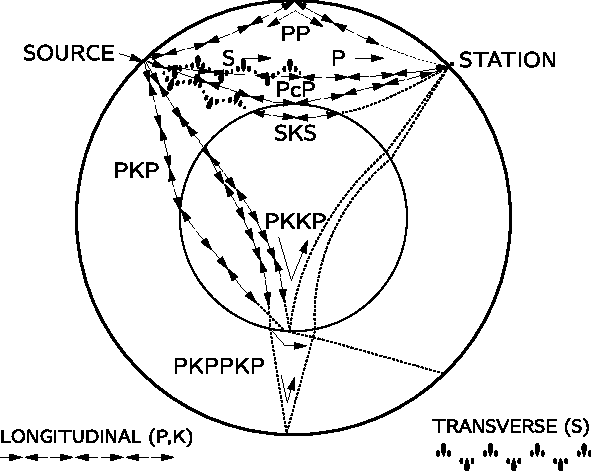
\includegraphics[width=0.9\linewidth]{fyz_fig0391.pdf}
    \caption{Schématické znázornění Země, na kterém jsou vidět dráhy podélných a příčných zvukových 
             vln
             (\cite[s.~690]{Feynman01})}
    \label{fyz:fig0391}
  \end{figure}
  
  V souvislosti se zvukovou vlnou si můžeme položit zajímavou otázku: Co se stane, když budeme 
  vlnovou délku v pevné látce stále zmenšovat? Kam až ji můžeme zkracovat? Je zajímavé, že nemůže 
  být kratší než vzdálenost mezi atomy. Předpokládáme-li totiž existenci vlny, v níž jeden bod se 
  pohybuje nahoru, druhý dolů atd., je nám jasné, že nejkratší možná vlnová délka je rovna 
  vzdálenosti mezi atomy. Mody můžeme klasifikovat, a tak známe podélné a příčné mody, dlouhovlnné 
  a krátkovlnné mody. Uvažujeme-li vlnové délky porovnatelné s meziatomovou vzdáleností, nejsou už 
  rychlosti konstantní; vzniká disperzní jev, kdy rychlost závisí na vlnovém čísle. Ale nejvyšším 
  modem příčných vln bude nakonec ten, při němž se každý atom chová opačně než s ním bezprostředně 
  sousedící atomy. 

  \begin{figure*} %\ref{fyz:fig0392}
    \centering
    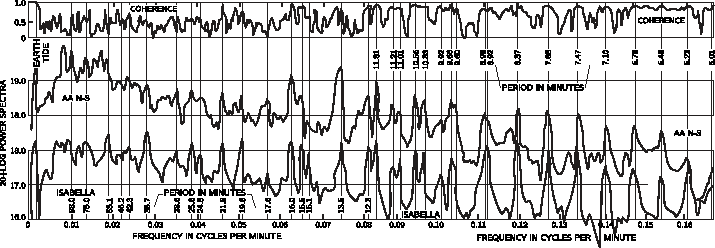
\includegraphics[width=1\linewidth]{fyz_fig0392.pdf}
    \caption{Závislost výkonu na frekvenci zaznamenaná seizmografy v Ñaña (Peru) a Isabella 
             (Kalifornie). Koherence udává míru vazby mezi oběma stanicemi. 
             (\cite[s.~693]{Feynman01})}
    \label{fyz:fig0392}
  \end{figure*}
  Z atomárního hlediska připomíná situace dvě vázaná kyvadla, o nichž jsme už mluvili a které mají 
  dva typy modů; v jednom případě se pohybují souhlasně, v druhém se pohybují proti sobě. Kmity v 
  pevných látkách můžeme tedy zkoumat i jinak, jako soustavu vázaných harmonických oscilátorů, jako 
  ohromné množství vázaných kyvadel, přičemž nejvyšší harmonická odpovídá situaci, kdy kmitají 
  proti sobě a nižší harmonické odpovídají jiným z fázováním. 
  
  Nejkratší vlnové délky jsou tak krátké, že nejsou obvykle technicky dosažitelné. Mají však velký 
  význam, neboť v termodynamické teorii pevných látek můžeme analyzovat tepelné vlastnosti látek 
  například jejich tepelné kapacity pomocí vlastností krátkých zvukových vln. Přechod k extrémně 
  krátkým vlnovým délkám zvukových vln nezbytně vede k individuálním pohybům atomů; tyto dvě věci 
  jsou v konečném důsledku totožné. 

  Velmi zajímavým příkladem zvukových vln v pevném tělese, podélných i příčných,jsou vlny, které se 
  šíří uvnitř Země. Nevíme, kdo vytváří tyto zvuky, ale uvnitř Země se čas od času projeví 
  zemětřesení - jedna hornina sklouzne po druhé. Je to jako slabý zvuk. Z takového zdroje se potom 
  začne šířit vlna podobná zvukové vlně. I když její vlnová délka je mnohem větší než vlnová délka 
  obyčejného zvuku, jsou to přece jen zvukové vlny a šíří se Zemí. Země však není homogenní a tlak, 
  hustota, stlačitelnost a jiné vlastnosti se mění s hloubkou, takže se mění s hloubkou i rychlost 
  vlny. Vlny proto nepostupují přímo - vzniká jistý druh indexu lomu a vlny se šíří křivočaře. 
  Podélné a příčné vlny mají jiné rychlosti a pro různé rychlosti máme různá řešení vlnové rovnice. 
  Umístíme-li někde \emph{seizmograf} a pozorujeme pohyb jehly po zemětřesení, které vzniklo na 
  některém jiném místě, neuvidíme jen nepravidelné chvění. Můžeme registrovat kmitání a ustálení a 
  další kmitání, a všechno, co se děje, závisí na poloze. Kdyby zemětřesení bylo velmi blízko, 
  nejprve by dorazily podélné vlny a o chvíli později příčné, protože postupují pomaleji. Měřením 
  časového rozdílu mezi těmito dvěma událostmi bychom zjistili vzdálenost ohniska zemětřesení, 
  pokud bychom dost věděli o rychlostech těchto vln a skladbě vnitřních částí Země.
  
  Na obrázku \ref{fyz:fig0391} je schematicky znázorněno chování vln uvnitř Země. Dva druhy vln jsou 
  označeny různými symboly. Kdyby v místě označeném jako zdroj došlo k zemětřesení, příčné a 
  podélné vlny, jdoucí k pozorovací stanici přímo, by dorazily v různých okamžicích a v důsledku 
  odrazu na nespojitostech by se objevily i jiné než přímé dráhy, a tedy i jiné okamžiky příchodu 
  vln. Ukazuje se, že v Zemi existuje jádro, které nevede příčné vlny. Je-li pozorovací stanice 
  proti zdroji, dojdou k ní příčné vlny, ale nesprávně načasované. Dochází totiž k tomu, že když 
  příčná vlna přichází na své cestě k jádru k šikmému povrchu mezi dvěma materiály, vznikají nové 
  vlny: jedna příčná a jedna podélná. V zemském jádře se však příčná vlna nešíří (aspoň na to 
  nemáme na rozdíl od podélných vln důkaz). Na druhé straně jádra podélná vlna opět vybudí vlny dvě 
  a ty přicházejí k pozorovací stanici.
  
  Právě z povahy vln vyvolaných zemětřesením se zjistilo, že příčné vlny se nemohou šířit v kulovém 
  objemu ve středu Země. To znamená, že střed Země je kapalný v tom smyslu, že nevede příčné vlny. 
  Jediným způsobem, kterým se dovídáme, co je uvnitř Země, je studium zemětřesení. Velkým počtem 
  pozorování mnoha zemětřesení v různých pozorovacích stanicích byly zjištěny všechny podrobnosti - 
  nyní už známe rychlosti vln, jejich dráhy, atd. Víme, jakými rychlostmi se šíří různé druhy vln v 
  libovolné hloubce. Když už známe rychlost šíření zvukových vln, můžeme vypočítat, jaké jsou 
  vibrační mody Země. Jinými slovy: známe elastické vlastnosti obou druhů vln v libovolné hloubce. 
  Předpokládejme, že se Země zdeformovala do tvaru elipsoidu a v této podobě zůstala. Abychom 
  určili periodu a tvar volného modu, stačí superponovat vlny šířící se elipsoidem. Už jsme 
  zjistili, že v případě poruchy se objeví množství modů, od nejnižšího, který je elipsoidální k 
  vyšším modům se složitější strukturou.
  
  Zemětřesení v Chile v květnu 1960 vyvolalo tak silný „šum“, že jeho signály mnohokrát obešly 
  Zemi. V této době už byly nainstalovány nové, velmi citlivé seizmografy, pomocí nichž bylo možno 
  určit základní mody Země a porovnat je s hodnotami vypočítanými z teorie zvuku pomocí rychlostí 
  změřených při jiných, nezávislých zemětřeseních. Výsledek takového experimentu je ilustrován na 
  obr. \ref{fyz:fig0392} ve formě závislosti síly signálu na jeho frekvenci (Fourierova analýza). Na 
  některých z přijímaných frekvencí jsou signály podstatně silnější, jsou tam určitá maxima. Ta 
  odpovídají vlastním frekvencím Země, jsou to hlavní frekvence, na nichž Země může kmitat. Je-li 
  celkový pohyb Země složen z modů mnoha frekvencí, můžeme pro každou stanici očekávat, že 
  nepravidelné výkyvy jsou superpozicí signálů mnoha frekvencí. Z jejich frekvenční analýzy bychom 
  mohli určit charakteristické frekvence Země. Svislé plné čáry na obrázku jsou vypočtené frekvence 
  a zjišťujeme pozoruhodnou shodu, která svědčí o tom, že teorie zvuku uvnitř Země platí.
  
  Velmi zajímavou skutečnost odhaluje obrázek \ref{fyz:fig0393}, na němž jsou znázorněny výsledky 
  velmi přesného měření s lepším rozlišením nejnižšího - elipsoidálního modu Země. Všimněme si, že 
  nejde o jednoduché, ale o zdvojené maximum, jehož vrcholy v \num{54.7} min. a \num{53.1} min. 
  jsou trochu posunuty. Příčina těchto dvou různých frekvencí nebyla v době jejich měření známá, 
  ale dnes už se na ni možná přišlo. Existují přinejmenším alespoň dvě možná vysvětlení. První z 
  nich vychází z možné asymetrie v rozložení zemské hmoty a ta by způsobila existenci dvou 
  podobných modů. Jiné, ještě zajímavější vysvětlení spočívá v následujícím. Představme si vlny, 
  které postupují od zdroje kolem Země ve dvou směrech. Jejich rychlosti nebudou stejné, neboť v 
  pohybových rovnicích figuruje otáčení Země, s nímž jsme dosud v analýzách nepočítali. Pohyb v 
  rotující soustavě je modifikován \emph{Coriolisovou silou} a to může způsobit pozorované 
  rozštěpení.

  \begin{figure}[ht!] %\ref{fyz:fig0393}
    \centering
    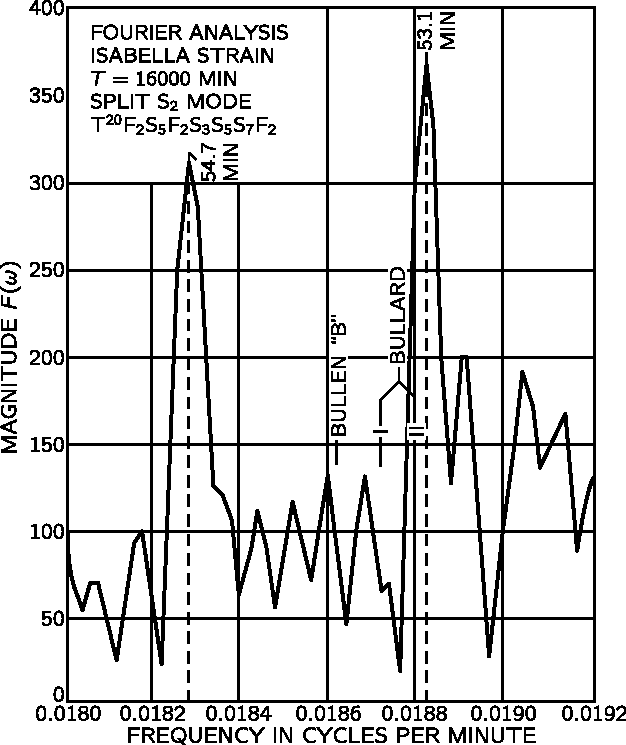
\includegraphics[width=0.6\linewidth]{fyz_fig0393.pdf}
    \caption{Analýza jednoho seizmografického záznamu s vysokým rozlišením ukazuje spektrální 
             dublet.
             (\cite[s.~694]{Feynman01})}
    \label{fyz:fig0393}
  \end{figure}
  
  Řekněme si ještě pár slovo metodě registrace takových otřesů. To, co zapisuje seizmograf, není 
  závislost amplitudy na frekvenci, ale závislost posunutí na čase, což zanechává velmi 
  nepravidelnou stopu. My, však už víme, co musíme udělat, abychom dostali podíl jednotlivých 
  sinových vln pro všechny frekvence. Získaný údaj musíme násobit sinovou vlnou dané frekvence a 
  integrovat, tj. vystředovat ji. Při tomto postupu ostatní frekvence vymizí. Na obrázcích jsou 
  vlastně znázorněny křivky integrálů z údajů násobených sinovými vlnami s různým počtem period za 
  minutu.
  
\section{Povrchové vlny}\label{fyz:IchapLIsecIV}
  Dalším zajímavým typem vln jsou vlny na vodě, které každý z nás určitě viděl a které bývají často 
  používány jako příklad vln v základních kursech. Jak brzy uvidíme, je to ten nejhorší příklad, 
  neboť tyto vlny vůbec nepřipomínají zvuk nebo světlo a vyznačují se všemi komplikacemi, které 
  vlny mohou mít. Uvažujme nejprve dlouhé vlny na hluboké vodě. Považujeme-li oceán za nekonečně 
  hluboký a na jeho povrchu vznikne rozruch, objeví se vlny. Vzniknou všechny druhy nepravidelných 
  pohybů, ale sinusoidální pohyb s velmi malou výchylkou může připomínat obyčejné hladké mořské 
  vlny postupující k pobřeží. V případě takových vln zůstává voda v průměru na místě a pohybuje se 
  pouze vlna. Položme si otázku: Jde o příčný nebo o podélný pohyb? Nemůže to být ani příčný, ani 
  podélný pohyb! I když v daném místě je voda střídavě v brázdě a na hřebenu, nemůže jít o 
  jednoduchý pohyb nahoru a dolů v důsledku zákona zachování množství vody. Kam by se totiž poděla 
  voda po klesání, když je nestlačitelná? Rychlost vln stlačení - tedy zvuku ve vodě - je mnohem, 
  mnohem větší a nebudeme nyní o nich mluvit. Vodu budeme považovat za nestlačitelnou a proto při 
  sestupování hřebene musí voda z této oblasti odcházet do stran. Ve skutečnosti dochází k tomu, že 
  vodní částice se v blízkosti hladiny pohybují přibližně po kružnicích. Člověk vznášející se 
  na gumovém kole by po příchodu hladkých vln zpozoroval kruhový pohyb okolních předmětů. Aby náš 
  zmatek byl dokonalý, máme co činit se směsí příčných a podélných vln. Ve větších hloubkách 
  probíhá pohyb po menších kružnicích a dostatečně hluboko už pohyb zaniká (obr. \ref{fyz:fig0394}).
  
  \begin{figure}[ht!] %\ref{fyz:fig0394}
    \centering
    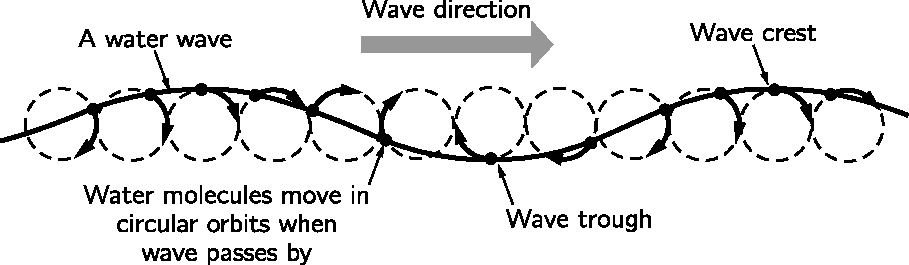
\includegraphics[width=0.95\linewidth]{fyz_fig0394.pdf}
    \caption{Vlny na hluboké vodě vznikají při pohybu částic po kružnicích. Všimněme si 
             systematického fázového posunu od jedné kružnice k druhé. Jak by se pohyboval 
             plavající předmět?
             (\cite[s.~695]{Feynman01})}
    \label{fyz:fig0394}
  \end{figure}

  Bude velmi zajímavé najít rychlost takových vln. Musí to být nějaká kombinace hustoty vody, 
  gravitačního zrychlení (gravitace je v tomto případě obnovující silou, která vytváří vlny) a 
  možná vlnové délky a hloubky. Ať už bude vztah pro fázovou rychlost vln jakýkoliv, musí to být 
  taková kombinace uvedených faktorů, která dá správný fyzikální rozměr. Budeme-li se o takovou 
  kombinaci pokoušet různými způsoby, jen jedním z nich bychom zkombinovali hustotu, \(g\) a 
  \(\lambda\) tak, abychom dostali rychlost a to je právě veličina \(\sqrt{g\lambda}\), která 
  hustotu vůbec neobsahuje. Tento výraz pro fázovou rychlost není vlastně zcela správný ale úplná 
  analýza dynamiky, kterou však nebudeme provádět, by nám poskytla vztah, který se od našeho liší o 
  bezrozměrný koeficient \(\sqrt{2\pi}\), takže
  \begin{equation*}
    v_{phase} = \sqrt{\dfrac{q\lambda}{2\pi}} \quad\text{(pro gravitační vlny)}.
  \end{equation*}
  Je zajímavé, že dlouhé vlny postupují rychleji než krátké. Vytvoří-li někde v dálce sportovní 
  motorový člun vlny, dorazí ke břehu nejprve vlny v podobě ojedinělých nárazů a pak budou tyto 
  nárazy častější a rychlejší, neboť jako první dorazily dlouhé vlny. Postupem času přicházejí 
  kratší a kratší vlny, neboť rychlost se chová jako druhá odmocnina z vlnové délky.
  
  Nyní možná namítneme, že k takovým úvahám potřebujeme znát grupovou rychlost. Budeme mít 
  samozřejmě pravdu. Vztah pro fázovou rychlost nám neřekne, co dorazí první; k tomu potřebujeme 
  znát grupovou rychlost. Musíme tedy určit grupovou rychlost a snadno si vypočítáme, že je rovna 
  polovině fázové rychlosti za předpokladu, že tato rychlost se chová jako druhá odmocnina z vlnové 
  délky. Grupová rychlost se také chová jako odmocnina z vlnové délky. Jak je možné, že grupová 
  rychlost je dvakrát menší než fázová rychlost? Všimněme si skupiny vln vytvářených člunem 
  plujícím vedle. Budeme-li sledovat některý hřeben zjistíme, že se pohybuje ve skupině vln kupředu 
  a postupně slábne až na čele úplně zanikne. V zadní části se nějak mysticky a tajuplně objevuje 
  malá vlnka, dere se dopředu a postupně sílí. Krátce řečeno, ve skupině se pohybují vlny, ale 
  samotná skupina vln se pohybuje jen poloviční rychlostí než je rychlost jednotlivých vln.
  
  \begin{figure}[ht!] %\ref{fyz:fig0395}
    \centering
    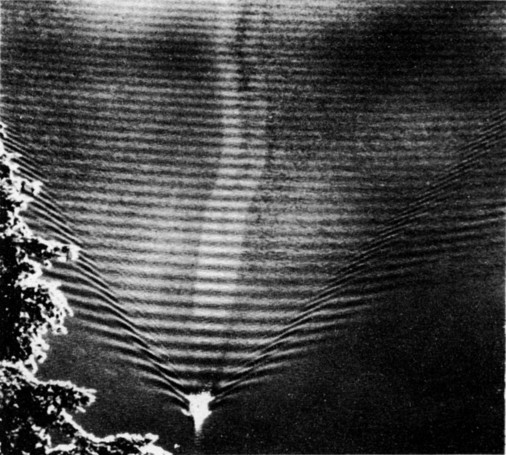
\includegraphics[width=0.6\linewidth]{fyz_fig0395.jpg}
    \caption{Brázda za člunem
             (\cite[s.~696]{Feynman01})}
    \label{fyz:fig0395}
  \end{figure}
  
  Protože grupová a fázová rychlost jsou rozdílné, nebudou vlny vytvářené pohybujícím se předmětem 
  kuželové, ale budou mít podstatně zajímavější tvar. Jaký tvar to bude je možné vidět z obrázku 
  \ref{fyz:fig0395}, který znázorňuje vlny vytvořené předmětem, pohybujícím se po vodě. Všimněme si, 
  že vlny vypadají zcela jinak než v případě zvuku, kdy rychlost nezávisí na vlnové délce. Ve 
  vzduchu byla čela vln jen podél kužele postupujícího do stran. Místo toho máme vlny vzadu, jejich 
  čela postupují souběžně s pohybem člunu a kromě nich máme vlnky po stranách postupující pod 
  jinými úhly. Tento složitý obrazec vln můžeme důvtipně analyzovat, jen když víme, že fázová 
  rychlost je úměrná druhé odmocnině z vlnové délky. Celý vtip spočívá v tom, že tento obraz vln je 
  stacionární vzhledem k člunu (pohybující se konstantní rychlostí). Jakýkoliv jiný obrazec vln při 
  pohybu člunu zmizí.
  
  Dosud jsme uvažovali dlouhé vlny, jejich obnovující silou byla gravitace. Jde-li však o velmi 
  krátké vlny ve vodě, jejich hlavní příčinou bude kapilární přitahování, tj. energie povrchového 
  napětí. Ukazuje se, že pro fázovou rychlost vln povrchového platí vztah
  \begin{equation*}
    v_{phase} = \sqrt{\dfrac{2\pi\sigma}{\lambda\varrho}}\quad\text{(pro vlnky)},
  \end{equation*}
  v němž \(\sigma\) označuje povrchové napětí a \(\varrho\) hustotu. Nyní máme opačnou situaci: 
  je-li vlnová délka malá, pak čím je vlnová délka kratší, tím je fázová rychlost \emph{větší}. 
  Máme-li i gravitaci i kapilární působení- což je vlastně běžné - musíme je zkombinovat a dostaneme
  \begin{equation*}
    v_{phase} = \sqrt{\dfrac{\sigma k}{\varrho} + \dfrac{g}{k}},
  \end{equation*}
  kde \(k = 2\pi/\lambda\) je vlnové číslo. Je vidět, že rychlost vln na vodě je opravdu složitá 
  věc.

  \begin{figure}[ht!] %\ref{fyz:fig0396}
    \centering
    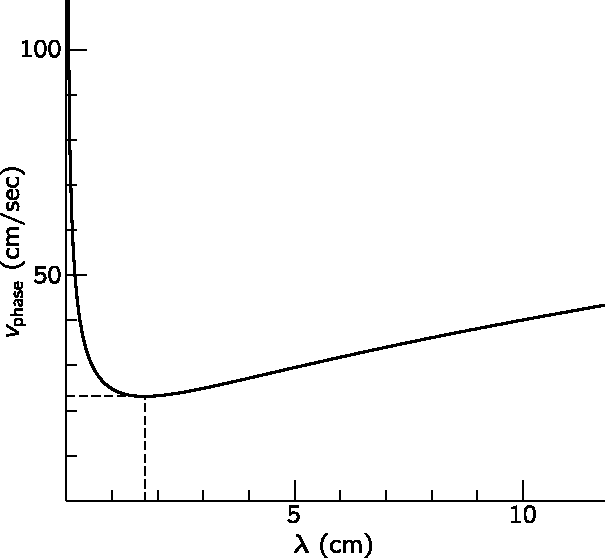
\includegraphics[width=0.6\linewidth]{fyz_fig0396.pdf}
    \caption{Závislost fázové rychlosti vlny na vodě na vlnové délce
             (\cite[s.~697]{Feynman01})}
    \label{fyz:fig0396}
  \end{figure}
  Obrázek \ref{fyz:fig0396} představuje fázovou rychlost jako funkci vlnové délky; pro velmi krátké 
  i velmi dlouhé vlny je velká a mezi těmito oblastmi existuje minimální rychlost šíření vln. 
  Kdybychom vycházeli z tohoto vztahu, mohli bychom určit i grupovou rychlost; v případě vlnek je 
  rovna \num{3/2} fázové rychlosti a v případě gravitačních vln \num{1/2} fázové rychlosti. Vlevo 
  od minima je grupová rychlost větší  než fázová, vpravo je tomu naopak. S těmito skutečnostmi 
  souvisí několik zajímavých jevů. Protože grupová rychlost roste velmi rychle s poklesem vlnové 
  délky, pak kdybychom vyvolali určitý rozruch, vznikly by vlny příslušné délky, šířící se 
  minimální rychlostí a před nimi by postupovaly rychlejší krátké a velmi dlouhé vlny. Ve vodní 
  nádrži snadno zpozorujeme krátké vln, ale jen těžko uvidíme dlouhé vlny. 
  
  Dozvěděli jsme se, že vlnky, které se tak často používají k ilustraci jednoduchých vln, jsou 
  vlastně složité a velmi zajímavé. Vůbec nemají strmá čela jako zvukové a světelné vlny. Kromě 
  hlavní vlny jsou zde vlny, které vybíhají dopředu. Ostrý rozruch ve vodě nevyvolává ostrou vlnu 
  právě v důsledku disperze. Nejprve přicházejí velmi drobné vlnky. Pohybuje-li se předmět ve vodě 
  určitou rychlostí, vzniká složitý obrazec, neboť různé vlny se pohybují různými rychlostmi. Na 
  tácku s vodou můžeme ukázat, že nejrychlejší jsou drobné kapilární vlny a vzadu postupují ty 
  nejpomalejší. Nakloníme-li dno, zjistíme, že tam, kde je malá hloubka vody, je menší i rychlost 
  vln. Postupuje-li vlna pod určitým úhlem vzhledem k přímce maximálního sklonu, ohýbá se směrem k 
  této přímce a má tendenci se pohybovat podél ní. Takovým způsobem se můžeme přesvědčit o mnoha 
  zvláštnostech vln na vodě a dojít k poznatku, že jsou mnohem složitější než vlny ve vzduchu. 


  \begin{figure}[ht!] %\ref{fyz:fig0397}
    \centering
    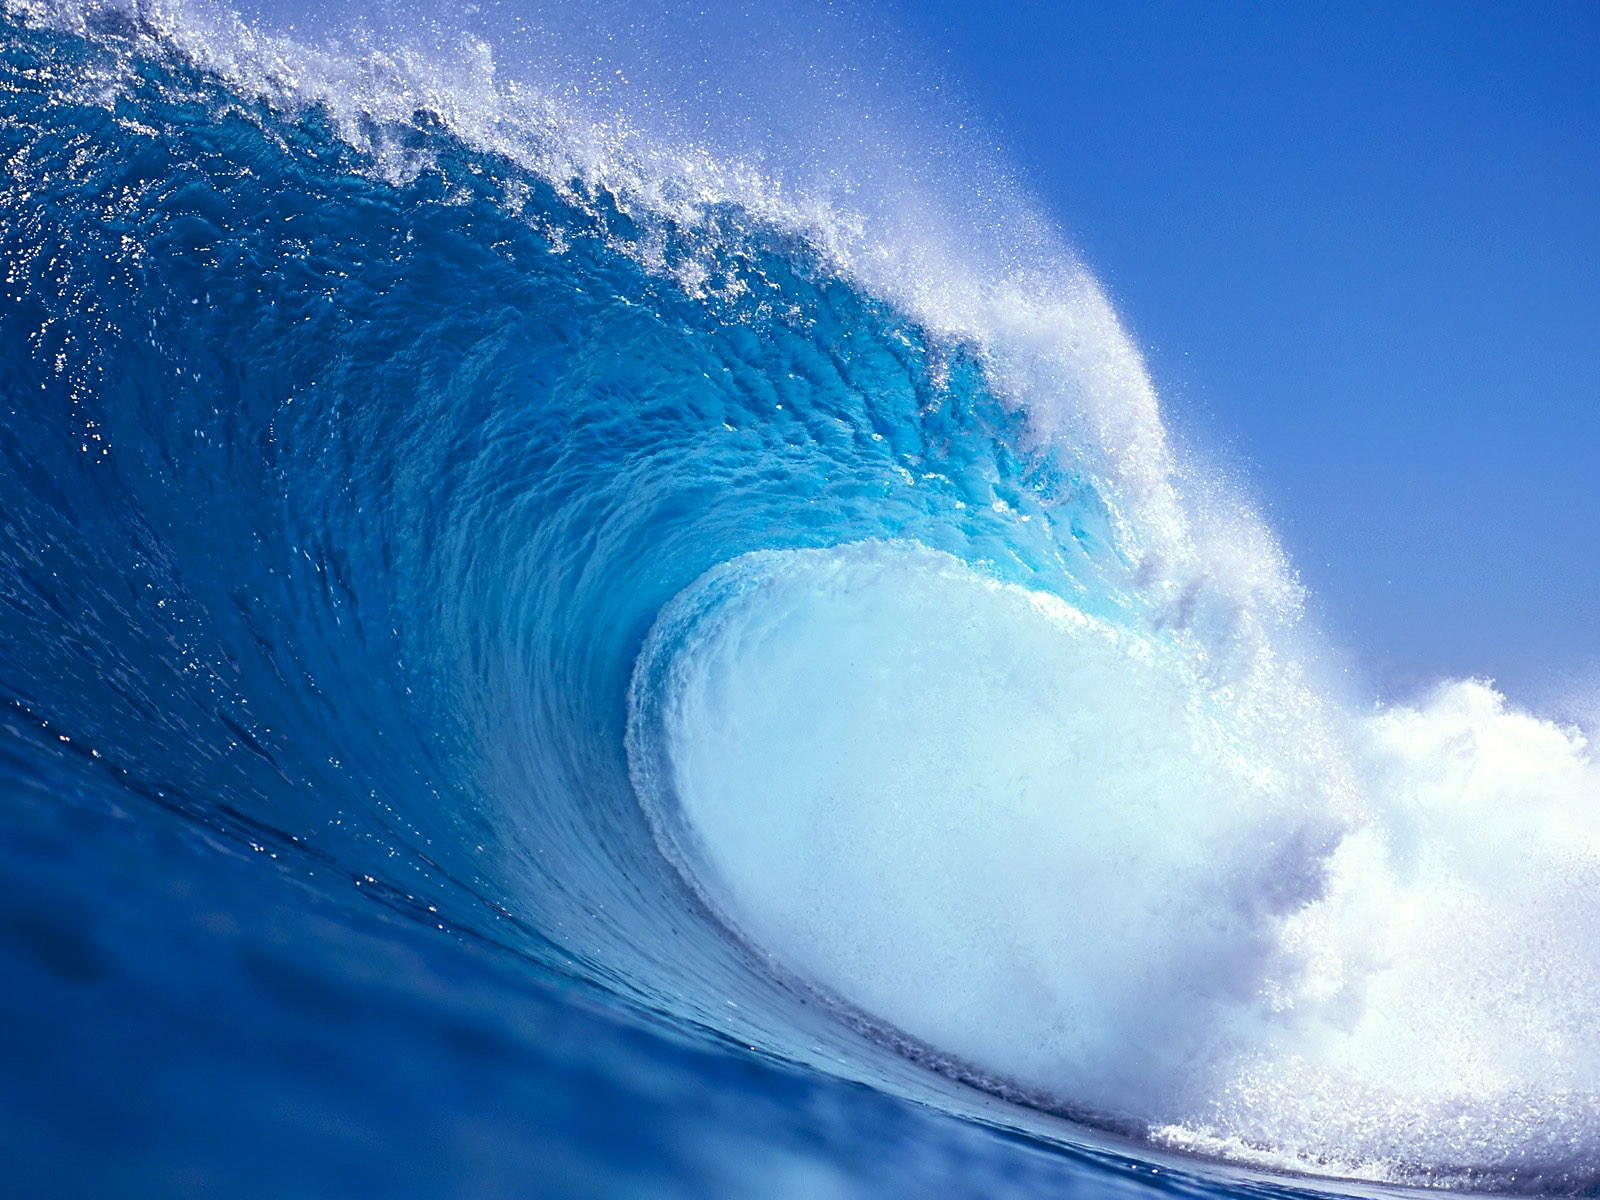
\includegraphics[width=0.6\linewidth]{fyz_fig0397a.jpg}
    \caption{Vlna na vodě
             (\cite[s.~697]{Feynman01})}
    \label{fyz:fig0397}
  \end{figure}
  
  Rychlost dlouhých vodních vln s cirkulačním pohybem je menší při menší hloubce a větší při větší 
  hloubce vody. Proto se vlna zpomalí, když se přiblíží k pobřeží, kde je mělčí voda. V hlubší vodě 
  se vlna pohybuje rychleji, a proto se objeví mechanizmus rázové vlny. Tentokrát, protože vlna 
  není tak jednoduchá, rázová vlna je deformovaná a hřeben vlny se láme známým způsobem zobrazeným 
  na obrázku \ref{fyz:fig0397} S takovou situací se setkáváme, když vlna dorazí ke břehu a poodhalí 
  ohromnou složitost přírody. Tvar vln se určí snadno, když jsou malé, ale když vzrostou a lámou 
  se, je to velice složité. 
  
  Zajímavou vlastnost kapilárních vln můžeme pozorovat, je-li vodní hladina porušena pohybujícím se 
  předmětem. Z hlediska samotného předmětu proudí voda kolem něho a vlny, které v konečném důsledku 
  zůstanou s ním, jsou vždy ty, které mají pravě takovou rychlost, aby se vzhledem k předmětu 
  nepohybovaly. Podobně budou vlny v okolí nehybného předmětu obtékaného proudem vytvářet 
  stacionární obrazec a budou to ty vlny, které mají stejnou rychlost jako obtékající voda. Je-li 
  však grupová rychlost menší než fázová, porucha postupuje v proudu nazpět, protože grupová 
  rychlost ji nestačí udržet v proudu. Je-li grupová rychlost větší než fázová, objeví se vlnový 
  obrazec před předmětem. Když se pozorně zahledíme na předmět v proudu, zpozorujeme drobné vlnky 
  před ním a dlouhé vzadu. 
  
  Jiný zajímavý jev podobného druhu je možno pozorovat při lití kapalin. Vyléváme-li například z 
  láhve dostatečně rychle mléko, zpozorujeme veliké množství čar křižujících se ve vytékajícím 
  proudu. Jsou to vlny vyvolané poruchou na okrajích a velice se podobají vlnám, pocházejícím od 
  předmětu nacházejícího se v proudu. Teď však jev vzniká po obou stranách, a tak se tvoří 
  křižující se čáry. 
  
  Seznámili jsme se s některými zajímavými vlastnostmi vln, s komplikacemi, které vznikají jako 
  důsledek toho, že fázová rychlost závisí na vlnové délce, rychlost vln na hloubce vody atd., a 
  které dělají přírodní jevy skutečně komplexními, a proto i zajímavými.
  
\section{Příklady a cvičení}\label{fyz:IchapLIsecVI}
  
  
%} %tikzset
%~~~~~~~~~~~~~~~~~~~~~~~~~~~~~~~~~~~~~~~~~~~~~~~~~~~~~~~~~~~~~~~~~~~~~~~~~~~~~~~~~~~~~~~~~~~~~~~~~~